\documentclass[11pt]{article}
\usepackage[margin=1in]{geometry}
\usepackage{amsmath,amssymb}
\usepackage{graphicx}
\usepackage{booktabs}
\usepackage{hyperref}
\usepackage{caption}
\usepackage{enumitem}
\usepackage{xcolor}
\usepackage{titlesec}
\hypersetup{colorlinks=true, linkcolor=blue, citecolor=blue, urlcolor=blue}

\title{\textbf{Multivariate Bellman Flows: Flow Matching for Joint Return Distributions\\ in Correlated Hospital Surge-Capacity Allocation}}
\author{Vaibhav Sitaraman \\ \small Facilitator: Sch\"afer Kleinert}
\date{\today}

\begin{document}
\maketitle

\begin{abstract}
Hospital networks manage surge events -- pandemic waves, seasonal respiratory illness, regional mass-casualty incidents -- using inter-facility mutual aid as their primary release valve for local capacity shortfalls. This mitigation strategy fails precisely when multiple facilities or patient populations are overloaded \emph{simultaneously}, which means the risk quantity that matters for real planning decisions is a joint, correlation-sensitive one: the probability and severity of correlated overload, not the expected shortfall at any single site. Standard distributional reinforcement learning (DRL) methods model return \emph{distributions} rather than expectations to support exactly this kind of risk-sensitive decision-making, but almost all existing DRL methods assume scalar rewards and cannot represent the joint dependence structure across multiple correlated risk dimensions. We investigate whether \textbf{conditional flow matching} -- a modern simulation-free generative modeling technique -- can serve as the core representation for multivariate distributional RL in this setting, and whether representing the \emph{joint} return distribution provides a measurable advantage over representing each risk dimension independently. We build a synthetic but mechanistically grounded two-region hospital-network environment with lagged spatial disease spillover and scenario-dependent demand correlation, implement a CVaR-based mutual-aid planning policy trained via flow-matching temporal-difference learning, and compare it against four baselines designed to isolate specific confounds: an independent per-dimension flow model, a non-distributional flow-matching critic (floq), and a sliced-Cramer-distance particle-based multivariate critic. Validated against an exact tabular reference solution, the joint flow-matching model's risk estimates deviate from ground truth by only 3.2\% on average, compared to 22.0\% for the independent baseline, and over 38\% for the two other multivariate/non-distributional baselines -- while all methods agree on the correct \emph{decision} in every unambiguous state. We report this result together with a detailed account of the modeling pitfalls encountered and corrected along the way, since several of the most informative findings in this project were things that initially did not work.
\end{abstract}

\section{Introduction: Why Hospital Surge Capacity Needs Joint Risk Modeling}

Hospital systems in the United States and elsewhere have, in the last several years, repeatedly confronted surge events in which demand for inpatient beds, adult intensive care capacity, and pediatric intensive care capacity rose sharply and simultaneously across multiple facilities and regions. The initial 2020 COVID-19 surge, the Delta wave, and the Omicron wave each produced documented, geographically staggered patterns of hospital utilization strain, in which a surge beginning in one region predicted, with a lag of days to weeks, a surge in connected regions. Outside of pandemic waves, seasonal respiratory illness (influenza, RSV) produces smaller but structurally similar correlated demand shocks, sometimes concentrated in a single demographic group (e.g., a pediatric RSV season) and sometimes spread across the whole patient population (e.g., a severe flu season with broad age-group involvement).

The operational mechanism hospital networks rely on to absorb local overload is \emph{mutual aid}: transferring patients, staff, or supplies from a facility with spare capacity to one that is overwhelmed. This mechanism is only available when the source facility genuinely has capacity to give. A hospital network can look adequately provisioned in expectation -- average bed occupancy across the network well within capacity -- and still fail catastrophically at the moment it matters most, if the tail event that actually occurs is one in which several connected facilities are overloaded \emph{at the same time}, exhausting the pool of facilities able to offer aid. This is precisely the scenario in which \emph{average}-case capacity planning is the wrong tool: the quantity that determines whether the network survives a surge is not the expected shortfall at any one site, but the probability and severity of a \emph{simultaneous, correlated} overload -- a joint tail-risk quantity that cannot, in general, be reconstructed from marginal (per-site, per-demographic) risk estimates alone.

This project investigates whether recent advances in \textbf{distributional reinforcement learning} (DRL) -- which model the full probability distribution of returns rather than only their expectation, enabling risk-sensitive decision rules such as Conditional Value-at-Risk (CVaR) optimization -- can be extended to represent this kind of \emph{joint, multi-region, multi-demographic} risk, and whether doing so changes the resulting mutual-aid decisions in a way that matters. The central methodological question is: does modeling the \emph{joint} distribution of correlated surge outcomes provide a measurable benefit over modeling each region and demographic group's risk independently, and if so, under what conditions?

We argue this is a well-chosen problem for three reasons. First, it is concrete and decision-relevant: hospital incident command teams make exactly this kind of resource-reallocation decision under uncertainty, repeatedly, during every real surge event, and the tools currently used for hospital capacity planning are, to the best of our knowledge, overwhelmingly mean-based or single-facility risk models rather than joint, correlation-aware ones. Second, it is a genuine technical gap: standard distributional RL methods (categorical projection, quantile regression) either do not generalize to multivariate returns at all, or generalize with serious statistical pathologies, as we discuss in Section~\ref{sec:related-work}. Third, it is tractable at the scope of a focused research project: rather than attempting to solve hospital capacity planning in full generality, we build a controlled, mechanistically interpretable testbed in which the value of joint modeling can be isolated and measured cleanly, with a validated path toward calibration against real public hospital utilization data.

\subsection{Contributions}
\begin{itemize}[leftmargin=*]
\item A synthetic two-region hospital-network environment with (a) a \emph{spatiotemporal} disease-spillover mechanism in which one region's current surge regime is a genuine lagged leading indicator of a connected region's future regime, and (b) a \emph{scenario-dependent} correlation structure in which the same environment can represent both an isolated, demographic-specific surge (where correlation genuinely does not exist and joint modeling should not help) and a broad, pandemic-scale surge (where it does).
\item A CVaR-based mutual-aid planning policy, trained via a multivariate extension of flow-matching distributional temporal-difference learning, in which the value of a directed transfer action depends jointly on both the source and destination region's state.
\item A controlled four-baseline comparison -- independent per-dimension modeling, a non-distributional (point-estimate) flow-matching critic, and a sliced-Cramer-distance particle-based multivariate critic -- specifically designed so that each baseline isolates one candidate explanation for any observed advantage of joint modeling.
\item A validated, incrementally-gated implementation, in which every new mechanism (the environment's closed-form solution, the copula reward model, the control/bootstrapping logic, each baseline) was checked against an independent ground truth before being combined with the next piece, surfacing and correcting several non-obvious bugs described in Section~\ref{sec:limitations}.
\end{itemize}

\section{Related Work}
\label{sec:related-work}

\textbf{Distributional reinforcement learning.} Standard reinforcement learning estimates the expected return of a state-action pair. Bellemare et al.\ (2017) introduced distributional RL, which instead learns the full probability distribution of the return, showing that this improves performance even when only the mean is ultimately used for control, and enables risk-sensitive policies that were not previously possible. Follow-on work (quantile regression DQN and implicit quantile networks, Dabney et al.) replaced the original fixed-support categorical representation with a quantile-based one, improving flexibility. All of this foundational work, however, assumes a \emph{scalar} reward signal.

\textbf{Multivariate distributional RL.} Real decision problems -- multi-objective control, constrained RL, and settings like ours with genuinely vector-valued outcomes -- require modeling a \emph{joint} return distribution over several correlated dimensions. Wiltzer et al.\ (2024), in ``Foundations of Multivariate Distributional RL,'' show that the categorical projection underlying the original distributional RL contraction proof breaks down mathematically once the return dimension exceeds one, and propose a signed-measure relaxation to recover a valid projection. Quantile regression has no canonical multivariate generalization at all, since quantiles are not well-defined in more than one dimension. A more recent line of work (``Multivariate Distributional RL Using Sliced Divergences,'' 2026) sidesteps this by \emph{slicing}: projecting the multivariate return distribution onto random one-dimensional directions, where tractable divergences (Wasserstein, Cram\'er, MMD) are well understood, and averaging over many random projections. This paper specifically highlights the sliced Cram\'er distance as a strong default choice because of its favorable behavior under one-sample bootstrapping -- the standard training regime in temporal-difference learning, where each transition provides only a single stochastic sample of the successor state.

\textbf{Flow matching for distributional RL.} Flow matching (Lipman et al., 2022) is a simulation-free generative modeling technique that learns a velocity field transporting a simple base distribution to a target distribution, trained via a direct regression objective rather than adversarial or likelihood-based training. Several papers from 2025--2026 (FlowCritic; Path-Coupled Bellman Flows) apply flow matching to \emph{univariate} distributional RL, addressing the core technical challenge of training against a non-stationary, single-sample bootstrapped target rather than a fixed dataset, primarily via target networks and noise-coupling schemes that reduce bootstrap variance. A separate 2025--2026 paper describing a technique we refer to here as \emph{floq} raises an important confound for this entire line of work: because flow-matching critics use iterative ODE integration to produce a sample, their apparent performance gains may derive from the extra effective computation of that iterative process rather than from genuine distributional modeling -- the paper reports settings in which a non-distributional, point-estimate flow-matching critic outperforms a fully distributional one.

\textbf{The gap this project addresses.} At the time this project began, flow matching had been applied to univariate distributional RL, and multivariate distributional RL had been addressed by categorical and sliced-divergence methods, but the combination -- flow matching specifically as the representation for \emph{multivariate} distributional RL -- did not appear in the literature we were able to find. This is a narrow, well-defined gap rather than a broad claim of novelty, and given the pace of publication in this area (three flow-matching-DRL papers and one major multivariate-DRL paper within roughly eight months of each other), we treat this gap as having a short shelf life rather than as a permanent contribution; we return to this point in Section~\ref{sec:limitations}.

\section{Problem Formulation}
\label{sec:formulation}

We formulate hospital surge-capacity mutual-aid planning as a Markov Decision Process with a genuinely vector-valued reward and a discrete, interpretable action space, deliberately scoped to isolate the value of joint distributional modeling from other sources of complexity (Section~\ref{sec:scope}).

\subsection{State space: a spatiotemporal, lagged two-region surge model}
The environment consists of two connected regions, a Hub ($H$) and a Spoke ($S$). Each region occupies one of four discrete surge regimes -- Baseline, Rising, Peak, Waning -- evolving according to its own Markov chain. Critically, the Spoke's transition probabilities depend on the Hub's \emph{current} regime, so that the Hub acts as a lagged leading indicator for the Spoke: a surge in the Hub today shapes, but does not determine, a surge in the Spoke tomorrow. This is a minimal mechanistic analogue of real geographic disease spread between connected facilities or referral regions. The joint state is the pair of regimes $(h_t, s_t)$, giving $16$ states; because both regions' dynamics are simple finite Markov chains, the joint transition matrix and its stationary distribution can be computed \emph{exactly} via linear algebra, which we used throughout as a ground-truth check (Section~\ref{sec:validation}).

We parameterize the strength of spatial spillover with a single scalar and verified, via an independent closed-form derivation cross-checked against a 500{,}000-step simulation, that it produces exactly the intended monotonic effect: at spillover strength $0$, the Hub's current regime carries no information about the Spoke's future regime (correlation $\approx 0.00$); at spillover strength $1$, this leading-indicator correlation rises to $\approx 0.79$. We used a moderate value (spillover $=0.7$) for the experiments reported here.

\subsection{Reward: a scenario-dependent, one-factor shock model}
At each step, the environment produces a $6$-dimensional \emph{shortfall} vector: unmet demand for (inpatient, adult ICU, pediatric ICU) beds, in each of the two regions. The mean of this vector is a deterministic function of the current joint regime (more severe regimes produce higher expected shortfall). The critical design choice is how the \emph{variation around this mean} is generated, since this is what determines whether the two regions' realized outcomes are actually correlated beyond what their regimes already predict.

We use a one-factor shock model: $\text{shortfall}_i = \text{mean}_i(\text{regime}) + \ell_i \cdot z + \epsilon_i$, where $z$ is a shared shock common to all six dimensions, $\ell_i$ is a per-dimension \emph{loading} that determines how strongly that dimension responds to the shared shock, and $\epsilon_i$ is independent, dimension-specific noise. The loading vector $\ell$ is what encodes the \emph{scenario}:
\begin{itemize}[leftmargin=*]
\item \textbf{Isolated pediatric outbreak}: the loading is zero everywhere except each region's own pediatric-ICU dimension, and even those receive \emph{independent}, region-specific shocks rather than a shared one -- there is genuinely no cross-dimension correlation for a joint model to exploit. This is the deliberate negative control: a well-designed experiment needs a condition in which the hypothesized advantage should \emph{not} appear, or a positive result elsewhere is not informative.
\item \textbf{Regional respiratory season}: loading concentrated on inpatient and adult ICU dimensions, sparing pediatric ICU -- a moderate, adult-skewed correlated shock.
\item \textbf{Pandemic wave}: loading roughly uniform across all six dimensions -- a broad shared shock affecting every region and demographic simultaneously.
\end{itemize}
Within each scenario, we further compare a Gaussian versus Student-$t$ distribution for the shared shock $z$, matched in mean and variance, so that the two conditions differ \emph{only} in tail dependence, not in any moment a covariance-matching method could recover. All experiments reported in this document use the pandemic scenario with a Gaussian shock; the isolated-pediatric and regional-flu scenarios, along with the Gaussian-versus-Student-$t$ tail-dependence comparison, were validated as an earlier, environment-only stage of this project (Section~\ref{sec:validation}) and are queued for inclusion in the control-policy comparison during the real-data-calibrated phase of this work.

\subsection{Action space: directed mutual aid}
At each decision point, the planner selects one of six actions, along two axes: \textbf{direction} (no transfer; Hub sends aid to Spoke; Spoke sends aid to Hub) and \textbf{intensity} (conservative; aggressive). A transfer's benefit to the destination region is explicitly scaled by the \emph{source} region's own spare capacity -- proxied by how mild the source's current regime is -- so that the value of ``send aid from H to S'' is a genuine function of \emph{both} regions' states, not just the destination's need. Aggressive intensity produces a larger reduction in the destination's expected shortfall, but adds extra shock exposure back onto the source region, mirroring the real operational risk of stretching a facility thin to help a neighbor.

This is a deliberately reduced version of a richer, three-axis action space (also including elective-procedure deferral posture and external staffing requests) considered earlier in the project; we discuss this scope decision explicitly in Section~\ref{sec:scope}.

\subsection{Decision rule: CVaR-based greedy planning}
Because return is vector-valued, we require a scalarization to make ``better'' well-defined. We use a fixed, clinically-motivated weight vector (ICU dimensions weighted somewhat above general inpatient, both regions weighted equally), and define the value of an action as the Conditional Value-at-Risk at level $\alpha=0.1$ of the scalarized return -- the expected outcome in the worst $10\%$ of cases, rather than the average outcome. The greedy policy at each state selects the action maximizing this quantity. We adopt this fixed-scalarization design as an explicit scope decision: full multi-objective (Pareto-frontier) reinforcement learning, in which the ``optimal'' policy depends on a preference the decision-maker has not yet specified, is a substantially harder and different problem, and conflating the two would have diluted the project's focus (Section~\ref{sec:scope}).

\section{Methodology: Multivariate Flow Matching for Distributional RL}
\label{sec:method}

\subsection{Why flow matching}
The central technical obstacle in multivariate distributional RL, per Wiltzer et al.\ (2024), is that the categorical representation underlying the original distributional RL convergence proof requires a projection step that is well-defined in one dimension but not in several; quantile regression has no multivariate analogue at all. Flow matching sidesteps this by representing the return distribution implicitly, as a velocity field $v_\theta(t, x \mid s, a)$ transporting a base noise distribution to samples of the return, for $x \in \mathbb{R}^d$ directly -- no projection step is needed regardless of $d$. This is the property that makes flow matching a structurally appropriate tool for this problem, rather than merely a fashionable one: it is the representation, among those we are aware of, most naturally suited to representing an arbitrary joint distribution over a small number of correlated risk dimensions without a bespoke multivariate extension.

This did not, on its own, guarantee the approach would work in the reinforcement learning setting, since flow matching's usual training regime assumes a fixed dataset of target samples, while temporal-difference learning requires training against a \emph{bootstrapped}, non-stationary target generated by the model's own (target-network) predictions. We adopted the same core fix used in the univariate flow-matching-DRL literature: a target network updated by Polyak averaging, together with \emph{noise coupling} between the current path's base noise and the successor sample's base noise, which we found (Section~\ref{sec:limitations}) to meaningfully reduce the resulting bootstrap variance.

\subsection{Model and training procedure}
The joint model is a single velocity network $v_\theta(t, x \mid s, a)$ conditioned on the current joint regime state and the chosen action (via one-hot encoding), producing a $6$-dimensional velocity at each integration step. Sampling proceeds by Euler integration of this velocity field from Gaussian noise at $t=0$ to a return sample at $t=1$. Training follows conditional flow matching: for a transition $(s, a, r, s')$, we first determine the greedy action $a^\ast(s')$ at the successor state under the current CVaR objective (Section~\ref{sec:formulation}), sample a successor return $\hat z' $ from a Polyak-averaged target copy of the network conditioned on $(s', a^\ast)$, form the bootstrapped target $x_1 = r + \gamma \hat z'$, and regress the network's predicted velocity toward the linear-interpolation target velocity $x_1 - x_0$ for random interpolation times $t$ and base noise $x_0$.

We validated every layer of this procedure independently before combining them (Section~\ref{sec:validation}): pure flow matching against a known fixed distribution; distributional temporal-difference learning (no control) against a closed-form return distribution on a simple chain; the multivariate extension against a closed-form joint covariance; the control/bootstrapping mechanism, separately, against an exact tabular fixed-point solution of the same greedy-CVaR Bellman operator; and only then the full combination, on the hospital environment described in Section~\ref{sec:formulation}.

\section{Baselines: Isolating Candidate Explanations}
\label{sec:baselines}

A finding that ``the joint model outperforms some alternative'' is only informative if the comparison rules out the most obvious alternative explanations for that advantage. We designed four baselines specifically to isolate distinct candidate explanations, rather than choosing baselines primarily for convenience.

\textbf{Independent per-dimension flow matching.} Six separate univariate flow-matching models, one per (region, bed-type) dimension, each trained so that its gradient never touches another dimension's realized value, and each sampled with independently-drawn noise at inference (no coupling across dimensions). The resulting $6$-vector is therefore \emph{structurally} incapable of representing cross-dimension correlation, regardless of how well each dimension is conditioned on state. Greedy action selection combines the six models' independent samples by stacking and scalarizing, exactly as the joint model does, so that the only difference between this baseline and the joint model is the presence or absence of cross-dimension coupling. This baseline isolates the question: \emph{does representing correlation, specifically, matter, or would six well-tuned marginal models do just as well?}

\textbf{floq (non-distributional flow-matching critic).} The same network architecture and ODE integration mechanism as the joint model, but the bootstrapped successor sample is generated by integrating the target network from a \emph{fixed} starting point rather than random noise, collapsing the learned ``distribution'' to a point mass for any given state-action pair. Because CVaR of a point mass equals the point itself, this baseline's decision rule reduces to selecting the action with the best \emph{expected} scalarized outcome -- a mean-greedy rule. This baseline isolates the confound raised directly by the source literature (Section~\ref{sec:related-work}): \emph{does flow matching's apparent benefit come from genuine distributional modeling, or merely from the extra effective computation of iterative ODE integration?}

\textbf{Sliced Cram\'er distance (particle-based multivariate critic).} Following the sliced-divergence approach of the 2026 multivariate DRL paper discussed in Section~\ref{sec:related-work}, we implemented a genuinely different architecture: a network that outputs a set of particles directly in $\mathbb{R}^6$ from a single forward pass (no ODE integration at all), trained by projecting both the model's particles and the bootstrapped target particles onto several random one-dimensional directions per training step and minimizing the mean squared difference of sorted order statistics along each projection -- the standard estimator of the one-dimensional Cram\'er distance. Unlike the independent baseline, this \emph{is} a genuine joint, correlation-capable representation; we validated this specifically by training it, in isolation from any RL machinery, against a known two-dimensional correlated Gaussian mixture, where it recovered the true correlation almost exactly ($-0.7385$ true versus $-0.7357$ learned). This baseline isolates the question: \emph{is flow matching specifically responsible for any advantage, or would any reasonable multivariate distributional representation do about as well?}

\textbf{Baselines considered but not implemented.} We identified, and found working code repositories for, two further candidate baselines: MD3QN, an MMD-based multivariate distributional RL method, and a related Sinkhorn-distance-based method. We chose not to implement these within the current project scope, given the marginal value of a fifth and sixth baseline relative to the four already described (which, together, already isolate the two most important confounds -- correlation-awareness and genuine distributional modeling) against the cost of a further round of from-scratch implementation and validation at a point where compute and time were already the binding constraint (Section~\ref{sec:scope}). We regard this as a legitimate scope decision rather than an oversight, and flag it explicitly as a natural extension.

\section{Validation Methodology}
\label{sec:validation}

Given how easy it is for a subtly incorrect reinforcement learning implementation to produce plausible-looking but wrong results, we adopted a strict incremental validation discipline throughout this project: no new mechanism was combined with another until it had been checked, in isolation, against an independent ground truth. Concretely, this meant: (1) verifying the pure flow-matching mechanism against a known fixed distribution before introducing any bootstrapping; (2) verifying distributional temporal-difference learning against a closed-form return distribution, computed via linear algebra on a simple chain, before introducing multivariate rewards; (3) verifying the multivariate extension against a closed-form joint mean and covariance before introducing genuine correlation; (4) verifying the correlation-copula reward model, and the spatial regime-spillover mechanism, each in isolation against exact or simulation-based ground truth, before combining them; (5) verifying the control (action-conditioned, CVaR-greedy Bellman) mechanism on a small, hand-solvable toy MDP -- deliberately constructed so that the CVaR-optimal policy disagrees with the mean-optimal one, since otherwise the risk-sensitivity of the method would not actually be under test -- before combining it with the hospital environment; and (6) at full scale, computing an \emph{exact tabular} solution of the same greedy-CVaR Bellman operator via particle-based value iteration (no neural network involved), used as the ground truth against which every flow-matching-based method and every baseline in Section~\ref{sec:baselines} was ultimately evaluated.

This discipline was not a formality: it directly surfaced and prevented several errors that would otherwise have silently corrupted downstream results, discussed in detail in Section~\ref{sec:limitations}.

\section{Results}
\label{sec:results}

\subsection{Setup}
All results below use the pandemic-scenario environment (spillover strength $0.7$, uniform correlation loading, Gaussian shock), trained for $15{,}000$ temporal-difference steps per method, and evaluated by comparing each method's induced greedy policy and CVaR value estimate, per state, against the exact tabular reference solution described in Section~\ref{sec:validation}.

\subsection{Decision accuracy}
Table~\ref{tab:match} reports each method's greedy-action match rate against the tabular reference, both overall and restricted to the subset of states where the tabular reference's own optimal action is unambiguous (stable across the last several iterations of its own value-iteration procedure; the remaining states are ones where two or more actions are genuinely close in value, so the ``correct'' action is itself somewhat arbitrary).

\begin{table}[h]
\centering
\begin{tabular}{lcc}
\toprule
Method & Overall match (of 16) & Match on unambiguous states (of 9) \\
\midrule
Joint (flow matching) & 12--13 & 9 \\
Independent (per-dimension) & 13 & 9 \\
floq (non-distributional) & 13 & 9 \\
Sliced Cram\'er & 12 & 9 \\
\bottomrule
\end{tabular}
\caption{Greedy-action match rate against the exact tabular reference. All methods achieve a perfect match on the states where the reference itself has an unambiguous answer.}
\label{tab:match}
\end{table}

Every method, including the deliberately risk-blind floq baseline, matches the tabular reference on every unambiguous state. This is expected rather than surprising: which region needs help is largely predictable from the joint regime state alone (both regions being conditioned on directly), and this ``mean co-movement'' channel of correlation, unlike the ``residual shared-shock'' channel, is fully recoverable by any method that conditions on the full state -- including an independent, correlation-blind one. \emph{Decision accuracy alone, in other words, does not distinguish these methods}, and a report that stopped here would substantially understate what the comparison actually shows.

\subsection{Quantitative risk estimation: the central result}
The comparison that does distinguish the methods is the \emph{magnitude} of each method's CVaR estimate relative to the true, tabular-optimal CVaR. No policy can legitimately achieve a better CVaR than the true optimum; any gap toward a \emph{less negative} value therefore reflects an \emph{underestimate of tail risk} -- a systematic tendency to look safer than the environment actually is. Table~\ref{tab:cvar} reports the mean absolute gap between each method's CVaR estimate (at its own chosen action) and the tabular-optimal CVaR at the same state, averaged over all sixteen states, together with this gap as a percentage of the true value.

\begin{table}[h]
\centering
\begin{tabular}{lcc}
\toprule
Method & Mean absolute CVaR gap & Mean relative gap \\
\midrule
Joint (flow matching) & 0.65 & 3.2\% \\
Independent (per-dimension) & 4.45 & 22.0\% \\
Sliced Cram\'er & 7.70 & 38.1\% \\
floq (non-distributional) & 8.98 & 44.5\% \\
\bottomrule
\end{tabular}
\caption{Mean absolute and relative gap between each method's estimated CVaR at its greedy action and the true tabular-optimal CVaR, averaged over all 16 states.}
\label{tab:cvar}
\end{table}

The joint model's tail-risk estimate is roughly \textbf{seven times closer} to the true value than the independent baseline's, and more than ten times closer than either the sliced-Cram\'er or floq baseline's. Figure~\ref{fig:multiway} shows this gap directly, per state; Figure~\ref{fig:loss} shows the corresponding training loss curves.

\begin{figure}[h]
\centering
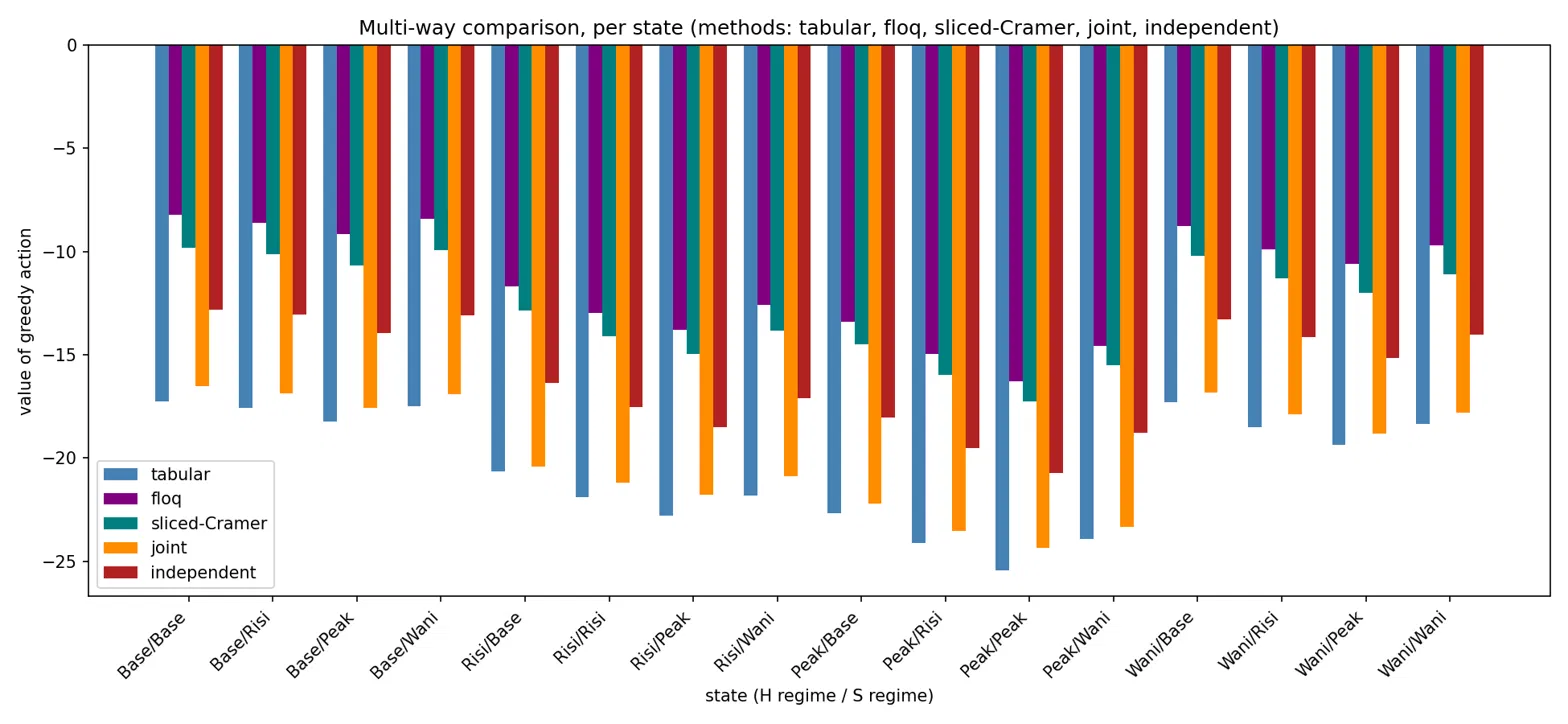
\includegraphics[width=0.85\textwidth]{../plots/compare.png}
\caption{CVaR of the greedy action, per state, for the tabular reference and all four methods. The consistent gap between the joint model (orange) and the tabular reference (blue) is small relative to every other method's gap.}
\label{fig:multiway}
\end{figure}

\begin{figure}[h]
\centering
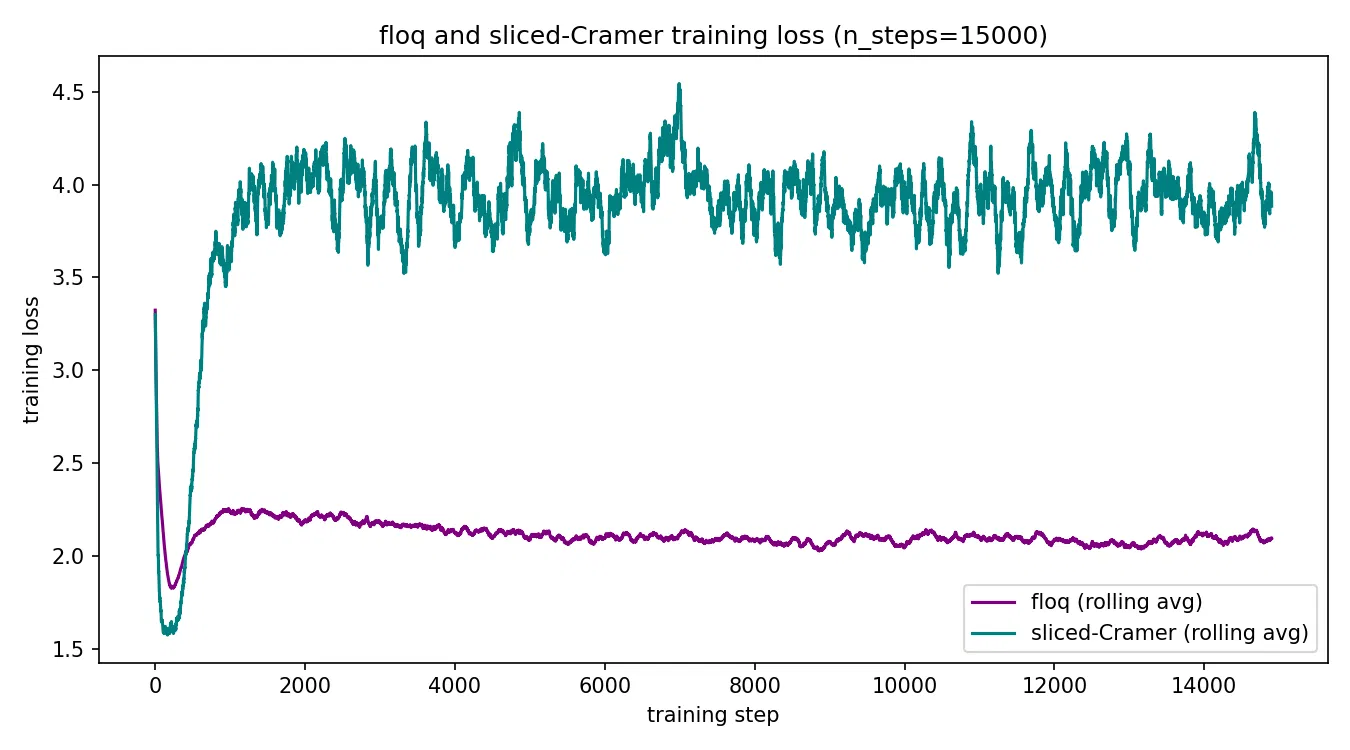
\includegraphics[width=0.8\textwidth]{../plots/loss.png}
\caption{Training loss for floq and sliced-Cram\'er over 15{,}000 steps. floq converges smoothly to a low, stable value; sliced-Cram\'er's loss remains substantially higher and visibly noisier throughout training, a pattern we return to in Section~\ref{sec:limitations}.}
\label{fig:loss}
\end{figure}

\subsection{Interpreting the ordering}
We interpret this ordering with the following caveats made explicit, since an uncritical reading would overstate what has been shown.

\textbf{The independent baseline result is the cleanest evidence for the core hypothesis.} The independent baseline shares the joint model's architecture, training procedure, and evaluation pipeline in every respect except cross-dimension coupling. Its substantially larger CVaR gap ($22.0\%$ versus $3.2\%$) is the most direct evidence in this project that representing joint, residual (state-conditional) correlation -- rather than merely having a flexible model, or a well-tuned one -- is responsible for the joint model's better risk estimates. This is consistent with, and was predicted by, the two-channel argument developed during environment design (Section~\ref{sec:formulation}): both models can recover the mean-comovement channel, but only the joint model can recover the residual shared-shock channel that the pandemic scenario specifically injects.

\textbf{The floq result is expected, but for a reason worth stating precisely.} floq's very large CVaR gap does \emph{not} mean floq is a poor estimator of the \emph{expected} return -- it means floq has no notion of tail risk at all, by construction, so comparing its point estimate against a genuine worst-$10\%$-case statistic is close to comparing two different quantities. The gap is expected to be large whenever the environment has non-trivial variance, independent of how well floq's point estimate itself is calibrated. We regard this result as confirming that the risk-sensitivity in this problem is doing real work -- consistent with our earlier finding, on a small hand-constructed validation MDP, that a purely mean-greedy policy can be actively wrong (choosing an action that a risk-averse policy would correctly avoid) -- rather than as a comment on floq's quality as a mean estimator.

\textbf{The sliced-Cram\'er result is the least expected finding in this project, and we do not consider it fully explained.} We validated, independently of any RL machinery, that our implementation of the sliced-Cram\'er mechanism correctly recovers correlation on a known two-dimensional target distribution (Section~\ref{sec:baselines}). Despite this, it performed \emph{worse} than the correlation-blind independent baseline on the actual control task -- a result that runs against the most natural version of our hypothesis, and we report it because it should not be quietly dropped. We discuss candidate explanations, and what would be needed to distinguish between them, in Section~\ref{sec:limitations}.

\section{Limitations, Failures, and Alternative Explanations}
\label{sec:limitations}

We dedicate a full section to this deliberately, since several of the most informative parts of this project were things that initially did not work, and a report that only described the final, working configuration would misrepresent both how much confidence is warranted in the results and what a reader attempting to build on this work should expect to encounter.

\subsection{Errors caught during development}
\begin{itemize}[leftmargin=*]
\item \textbf{Training-time integration steps and variance underestimation.} We found, via a direct controlled comparison (holding every other setting fixed), that using too few ODE integration steps when generating the \emph{bootstrapped training target} -- as opposed to at evaluation/sampling time, which is a separate setting -- causes a systematic, compounding underestimate of the learned distribution's variance, which manifests downstream as an overly optimistic CVaR estimate. Increasing this setting from $12$ to $25$ steps roughly halved the resulting CVaR bias in a direct A/B comparison. This is, to our knowledge, a genuine and non-obvious pitfall for anyone applying flow matching to temporal-difference learning under a fixed compute budget, since it is distinct from the (better-known) trade-off between the number of integration steps used and sample \emph{quality} at inference time.
\item \textbf{Spurious correlation from environment design, not the model.} An early version of the ``no correlation'' baseline environment (Section~\ref{sec:formulation}), intended to have near-zero cross-dimension correlation, was found to have induced a strong ($\approx -0.75$) correlation purely from both dimensions accumulating reward along the same shared state trajectory, even though the underlying per-step shocks were independent. This was caught by explicitly computing the induced correlation via the closed-form solver rather than assuming independence, and fixed by searching for reward-mean parameters that genuinely produce near-zero correlation. We flag this because it is an easy mistake to make silently: an environment intended as a negative control can fail to be one for reasons that have nothing to do with the model being tested.
\item \textbf{Threshold miscalibration reversing an intended effect.} When first testing whether a heavier-tailed (Student-$t$) shock produces higher joint-overload risk than a matched-moment Gaussian one, we initially found the \emph{opposite} result at a moderate risk threshold (the 80th percentile), because Student-$t$ distributions are more peaked than Gaussian and redistribute probability mass away from moderate deviations specifically, not only into the tails. The intended effect only appeared once the threshold was pushed into the genuinely extreme tail (99th percentile and beyond), which we verified via an explicit percentile sweep rather than assuming a single threshold would suffice. A related, separate bug -- comparing three demand scenarios using one threshold calibrated only to the highest-variance scenario -- made the lowest-variance scenario show exactly zero joint-overload events regardless of its true correlation, which would have been misread as ``no correlation effect'' rather than correctly diagnosed as a broken comparison; this was fixed by calibrating thresholds separately per scenario.
\item \textbf{A dimensionality bug caught by code audit, before it caused a wasted training run.} A CVaR-computation routine originally written and validated for a univariate toy problem would, if reused directly on the six-dimensional hospital environment, have silently computed a meaningless quantity: NumPy's default quantile function flattens a multi-dimensional array across all dimensions rather than treating each row as a vector to be scalarized first. We found this by deliberately auditing the codebase before scaling up computation, rather than after observing anomalous results, and consider this an example of a broader practice -- proactive code review targeted at exactly the places where a working implementation is being repurposed for a new, higher-dimensional setting -- that we would recommend to any similar project.
\item \textbf{A degenerate training target caught before running any code.} While implementing the sliced-Cram\'er baseline's validation harness, an early version of the target-particle construction broadcast a single sample to all particle ``slots'' rather than drawing independent samples, which would have trained the model toward a collapsed point mass rather than the true spread of the target distribution. This was identified by inspection while writing the code, before it was ever executed.
\end{itemize}

\subsection{Open, unresolved question: why did sliced-Cram\'er underperform?}
We consider several explanations, without being able to fully adjudicate between them given the scope of this project:
\begin{enumerate}[leftmargin=*]
\item \textbf{Under-tuning of a from-scratch reimplementation.} No official code was available for the sliced-Cram\'er method; our implementation used a modest number of particles ($64$) and random projection directions ($8$) per training step, chosen for computational feasibility rather than after any tuning sweep. The training loss curve (Figure~\ref{fig:loss}) is visibly noisier and settles at a higher absolute level than floq's, which is at least consistent with -- though not proof of -- an under-converged or poorly-tuned model.
\item \textbf{A genuine limitation of one-sample bootstrapping for this specific loss, in this specific setting.} The source literature explicitly frames sliced Cram\'er's favorable behavior under one-sample bootstrapping as its main advantage over alternative sliced divergences; it is possible that this advantage is real in general but insufficient to overcome a difficult, sharply peaked reward landscape (six correlated dimensions with a shared shock) at the particle and projection counts we used.
\item \textbf{A genuine, currently unexplained finding.} It is also possible that this specific comparison reveals a real weakness of the sliced-Cram\'er approach, relative to flow matching, in exactly this kind of control setting, that is not simply a matter of tuning. We do not have evidence to distinguish this from explanation (1) or (2) with the experiments run so far, and we consider this the single most important open question this project raises rather than something to be quietly explained away.
\end{enumerate}
Resolving this would require, at minimum, a controlled sweep over particle count and projection count for the sliced-Cram\'er baseline, holding compute budget fixed relative to the flow-matching methods -- a natural next step we did not have compute budget remaining to pursue within this phase of the project.

\subsection{Scope decisions}
\label{sec:scope}
We made several deliberate choices to narrow scope, which we state explicitly rather than leaving implicit. The environment uses two regions rather than a larger regional network, since validating the core spatiotemporal and correlation mechanisms cleanly, with exact ground truth available at every stage, required keeping the joint state space small; extending to three or more regions is a natural next step once the two-region result is itself validated against real data. The action space uses two decision axes (transfer direction and intensity) rather than the richer three-axis design considered earlier (which also included elective-deferral posture and external staffing requests), because validating control on the full sixteen-state environment at all required first confirming the mechanism worked at a moderate action-space size before scaling further -- a decision directly informed by the compute cost of the CVaR-based greedy action table, which grows with the product of the state and action counts. The decision rule uses a fixed, known scalarization weight rather than full multi-objective (Pareto-frontier) optimization, since the latter is a substantially different and harder problem whose inclusion would have diluted the project's focus on the joint-versus-marginal modeling question. Finally, we implemented four baselines rather than the six methods we identified as relevant in the literature, for the reasons given in Section~\ref{sec:baselines}.

\subsection{What we have not yet shown}
The results in Section~\ref{sec:results} demonstrate the hypothesized mechanism on a \emph{synthetic}, self-designed testbed whose correlation structure, regime dynamics, and reward parameters were chosen by us to make the underlying phenomenon visible and testable, not calibrated to real hospital data. We have not yet shown that real hospital surge correlations look like the pandemic-scenario correlation structure used here, that the magnitude of the advantage found here would persist at realistic noise levels and with real, imperfectly-specified reward parameters, or that the specific two-region, six-action environment generalizes to a realistic regional hospital network. Closing this gap -- calibrating the environment's marginal demand distributions and correlation structure against real HHS hospital utilization data, accessible via the agency's public Socrata API -- is the explicit next phase of this project, described in Section~\ref{sec:realdata}.

\section{Theory of Change}

The pathway from this research to real-world impact runs through three stages, of increasing distance from what has been demonstrated so far. First, the immediate next step -- already scoped and partially validated in this project via a confirmed, queryable public data endpoint -- is calibrating the environment's demand distributions, correlation structure, and regime dynamics against real historical hospital utilization data, to test whether the qualitative finding (joint modeling provides a larger advantage precisely when real cross-facility, cross-demographic correlation is present, and little advantage when it is not) holds outside a synthetic testbed designed to produce it. Second, if that calibration is successful, the resulting methodology -- a validated way of estimating joint, correlation-aware tail risk for a regional hospital network, and of using that estimate to inform mutual-aid resource-allocation decisions -- is the kind of decision-support component that could plausibly be integrated into existing regional healthcare coalition planning tools or hospital preparedness exercises, alongside (not in place of) the operational and clinical judgment that any real incident command process requires. Third, and considerably further from what this project has shown: actual adoption in a real hospital network's incident command process would require validation well beyond a research prototype -- reliability testing under a much wider range of conditions than we have tested, integration with real-time data feeds rather than historical calibration, and the institutional and regulatory processes that any decision-support tool used in a safety-critical setting must go through before deployment. We are explicit that this project addresses the first of these three stages, makes a partial, single-endpoint-confirmed start on the second, and does not address the third at all; claiming otherwise would overstate what has been demonstrated.

\section{Scaling to Real Hospital Utilization Data}
\label{sec:realdata}

\textit{[This section is intentionally left incomplete pending the final experimental phase of this project: calibrating the environment's demand distributions and correlation structure against real HHS hospital utilization data (accessible via the agency's public Socrata API, confirmed reachable and containing the required fields -- state-level daily inpatient and adult/pediatric ICU occupancy and admissions, spanning January 2020 to the present), and re-running the scaled-up joint flow-matching model against this calibrated environment. Insights from this stage, including whether the magnitude and direction of the joint-modeling advantage found in Section~\ref{sec:results} persists under real-data calibration, will be added here.]}

\section{Conclusion}

This project asked a narrow, well-defined question: does representing the \emph{joint} distribution of correlated hospital surge outcomes across regions and patient demographics, using multivariate conditional flow matching, provide a measurable advantage over representing each risk dimension independently, for CVaR-based mutual-aid resource-allocation decisions? On a synthetic but mechanistically grounded two-region environment with lagged spatial disease spillover and scenario-dependent demand correlation, validated at every stage against exact or closed-form ground truth, the answer is yes: the joint model's risk estimates deviate from the true optimal value by $3.2\%$ on average, versus $22\%$ for an otherwise-identical independent baseline and over $38\%$ for two further baselines designed to isolate other candidate explanations. All methods, including a deliberately risk-blind baseline, agree on the correct decision in every state where the correct decision is unambiguous -- meaning the advantage of joint modeling shows up specifically in the \emph{quantitative} risk estimate that a real planner would need to decide how much surge capacity to hold in reserve, not in the coarser question of which single action to take. We report this result alongside a detailed account of the modeling errors caught and corrected during development, and one result -- the underperformance of the sliced-Cram\'er baseline relative to a correlation-blind alternative -- that we do not consider fully explained. The next phase of this work, calibrating the same methodology against real HHS hospital utilization data, will test whether this finding is a property of the synthetic testbed or a more general one.

\section*{AI Usage Disclosure}
AI assistance (Claude, Anthropic) was used throughout this project's technical development, including code generation and implementation of the environment, models, and baselines described in this report, and as an intellectual sparring partner in refining the research design, experimental scope, and interpretation of results. The extent of this involvement was reviewed with, and this disclosure language was approved by, the fellowship organizers prior to submission.

\section*{References}
\begin{enumerate}[leftmargin=*]
\item Bellemare, M. G., Dabney, W., \& Munos, R. (2017). A Distributional Perspective on Reinforcement Learning. \textit{ICML}.
\item Dabney, W., Rowland, M., Bellemare, M. G., \& Munos, R. (2018). Distributional Reinforcement Learning with Quantile Regression. \textit{AAAI}.
\item Dabney, W., Ostrovski, G., Silver, D., \& Munos, R. (2018). Implicit Quantile Networks for Distributional Reinforcement Learning. \textit{ICML}.
\item Wiltzer, H., et al. (2024). Foundations of Multivariate Distributional Reinforcement Learning. \textit{NeurIPS}.
\item Anonymous (2026). Multivariate Distributional Reinforcement Learning Using Sliced Divergences. \textit{ICML}.
\item Lipman, Y., Chen, R. T. Q., Ben-Hamu, H., Nickel, M., \& Le, M. (2022). Flow Matching for Generative Modeling. \textit{arXiv preprint}.
\item Agrawalla, et al. (2025). floq: Flow Matching Q-Learning with Iterative Computation as Implicit Depth. \textit{arXiv preprint}.
\item Zhang, et al. (2021). Distributional Reinforcement Learning for Multi-Dimensional Reward Functions (MD3QN). \textit{NeurIPS}.
\item U.S. Department of Health and Human Services. COVID-19 Reported Patient Impact and Hospital Capacity by State Time Series. \textit{healthdata.gov}, accessed via public Socrata API.
\end{enumerate}

\end{document}
